\documentclass[10pt,twocolumn,letterpaper]{article}

\usepackage[T1]{fontenc}

\usepackage{cvpr}
\usepackage{times}
\usepackage{epsfig}
\usepackage{graphicx}
\usepackage{amsmath}
\usepackage{amssymb}

\usepackage{url}
\usepackage{hyperref}

% Include other packages here, before hyperref.

% If you comment hyperref and then uncomment it, you should delete
% egpaper.aux before re-running latex.  (Or just hit 'q' on the first latex
% run, let it finish, and you should be clear).
%\usepackage[pagebackref=true,breaklinks=true,letterpaper=true,colorlinks,bookmarks=false]{hyperref}

\cvprfinalcopy % *** Uncomment this line for the final submission

\def\cvprPaperID{****} % *** Enter the CVPR Paper ID here
\def\httilde{\mbox{\tt\raisebox{-.5ex}{\symbol{126}}}}

% Pages are numbered in submission mode, and unnumbered in camera-ready
\ifcvprfinal\pagestyle{empty}\fi
\begin{document}

%%%%%%%%% TITLE
\title{PC-2020/21 DES Finder Project}

\author{Lorenzo Arena\\
{\tt\small lorenzo.arena@stud.unifi.it}
}

\maketitle
\thispagestyle{empty}

%%%%%%%%% ABSTRACT
\begin{abstract}
    This project was made as the first work for the “Parallel Programming” exam
    at the University of Florence. The objective was to create two version of
    a software which, given a dictionary of passwords, could find the one matching
    a given combination of hash and salt; the first version had to be implemented
    as a sequential program, while the second had to be parallel, thus taking the
    advantages of multithreading.
    The encryption algorithm used was the DES used by the \verb|crypt| and
    \verb|crypt_r| Linux C functions (see \verb|man crypt|); for the ease of
    development another utility software has been created to generate both random
    or progressive dictionaries of passwords with the relative hashes and salts.
    The projects has been developed in C on a Ubuntu machine and all tests were made
    on a Intel i9-9900 CPU.
    The project is hosted on GitHub at
    \url{https://github.com/lorenzo-arena/des-finder-project}.
 \end{abstract}

 %%%%%%%%% BODY TEXT
\noindent\large\textbf{Future Distribution Permission}\\
\indent The author of this report gives permission for this document to be
        distributed to Unifi-affiliated students taking future courses.

\section{The sequential solution}

    The sequential solution has  a straightforward approach: it takes the hash
    and salt as the inputs, with an optional name for the dictionary file; then
    it starts reading the dictionary line by line, computing the hash and comparing
    it with the given one. Once a correspondence is found the program stops and
    prints the found password on the command line; if a correspondence is never
    found an error log is reported.

\section{The parallel solution}

    The parallel solution, implemented using C PThreads, uses one of the design
    patterns for multithreading solutions: \emph{producer} and \emph{consumers}.
    The program, as in the sequential solution, is started with a given hash and
    salt; optionally, the desired number of threads to use can be specified.
    The main thread then creates one \emph{producer} thread and the stated number of
    \emph{consumers} (or the maximum number for the CPU on which the software is running);
    then, using a barrier realized with a condition variable contained inside the
    search result structure, it waits until the password has been found or the entire
    dictionary has been processed.
    The \emph{producer} thread starts reading the dictionary file and fills a structure with
    a slice of the dictionary; once such structure has been filled the \emph{producer}
    appends the data to a queue and starts creating a new set of passwords taken
    from the dictionary.
    Each \emph{consumer} thread, when started, tries to get a set of passwords to compute on
    the queue, possibly waiting for a condition variable until the \emph{producer} has
    created a set for them; once a set is collected all the contained passwords are
    encpryted and checked against the original given hash, one by one:

    \begin{itemize}
        \item if they doesn’t match the thread tries to collect a new set
        \item if they match the thread signals the event to all the other threads,
              including the main one, using the condition variable on the search result
    \end{itemize}

\section{Results and observations}

    An extensive suite of tests has been conducted on a machine with a i9-9900 CPU;
    the dictionary used contained 5M passwords.
    The tests involved changing both the number of threads used and the position of
    the password in the dictionary; the times have been measured multiple times and
    averaged.
    The Figure \ref{fig:position} represents the trend of the time necessary to find the
    matching password on a given position for different threads numbers: most notably, the
    parallel solution with just 1 \emph{producer} and 1 \emph{consumer} threads is already
    better than the sequential solution because of the reading and computing split in
    different threads; we can also notice how for increasing number of threads the
    improvements in time start to reduce, or the performance even decreases (in the
    16 vs 15 threads case).

    \begin{figure*}
    \begin{center}
    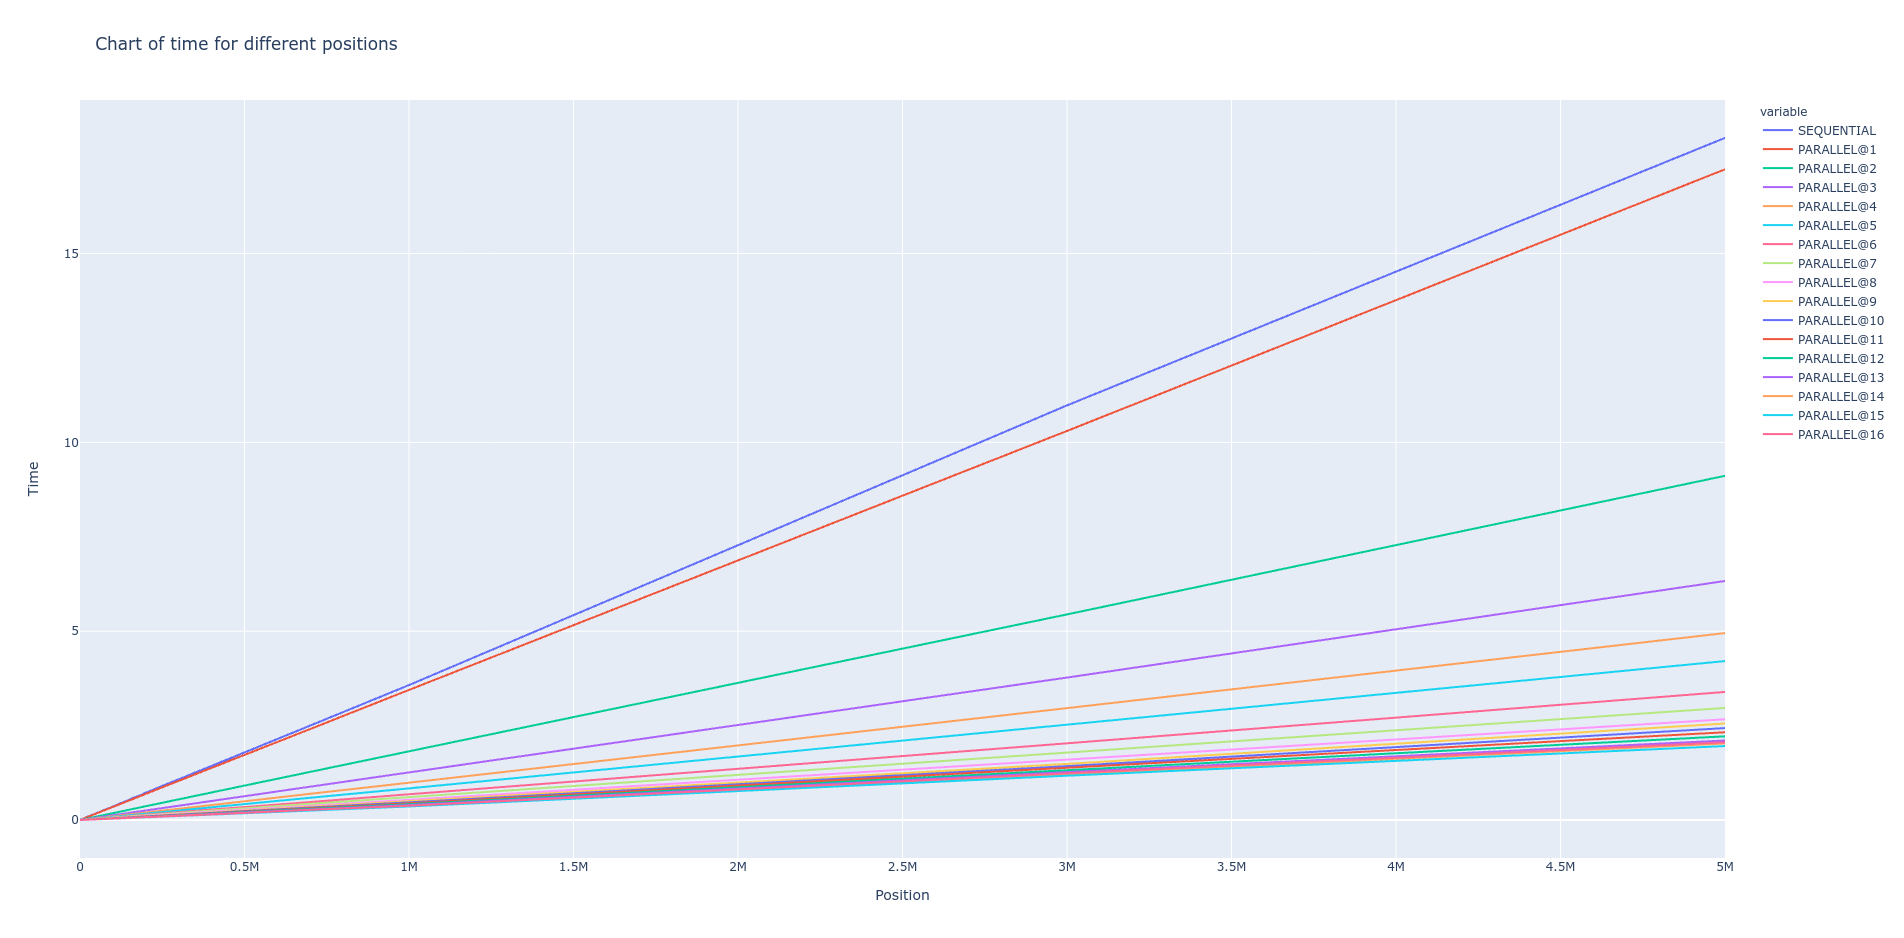
\includegraphics[width=1.0\linewidth]{./img/positions.png}
    \end{center}
        \caption{The times measured for different positions}
    \label{fig:position}
    \end{figure*}

    It’s also interesting to see how the different solutions behave when the password
    is found at the start of the dictionary (i.e. between the position 1 and 1000).
    From the tests it came out that the sequential solution is more efficient if the
    password is found in the first \textasciitilde350 positions; this is because the used size of
    each set of password created by the \emph{producer} thread is 300.
    Instead, the parallel solution run with a big number of threads (from 10 on) takes
    about three times the sequential solution time to find the password for the overhead
    related to thread management; this is rapidly pulled down by the time necessary for
    I/O operation (i.e. reading from the dictionary file) when the password is found
    after position \textasciitilde500.
    The chart for time necessary when password is found between position 1 and 10000 of
    the dictionary is showed in Figure \ref{fig:position-10k} and we can see that each line
    for the parallel solutions presents a periodical increase in the time; that is due to the
    fact that in some cases the password is found by a \emph{consumer} on the beginning of a set,
    while some other times it is found at the end.

    \begin{figure*}
    \begin{center}
    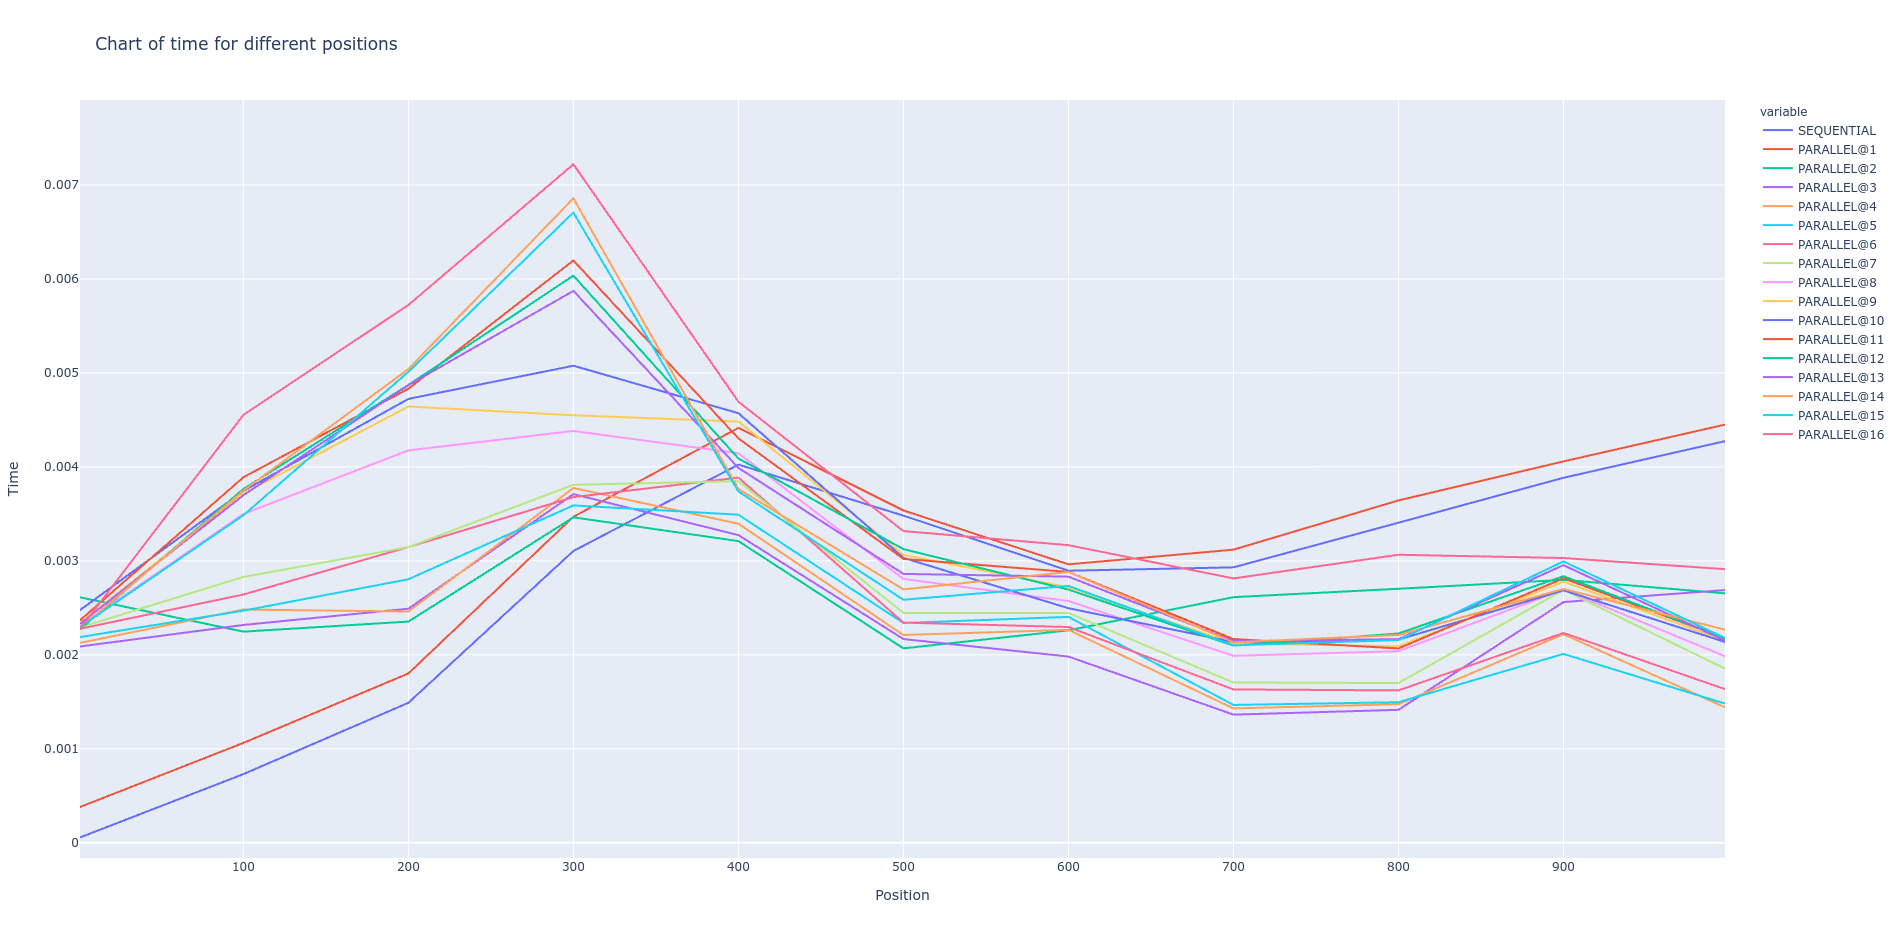
\includegraphics[width=1.0\linewidth]{./img/positions-1000.png}
    \end{center}
        \caption{The times measured for the first 1000 positions}
    \label{fig:position-1000}
    \end{figure*}

    \begin{figure*}
    \begin{center}
    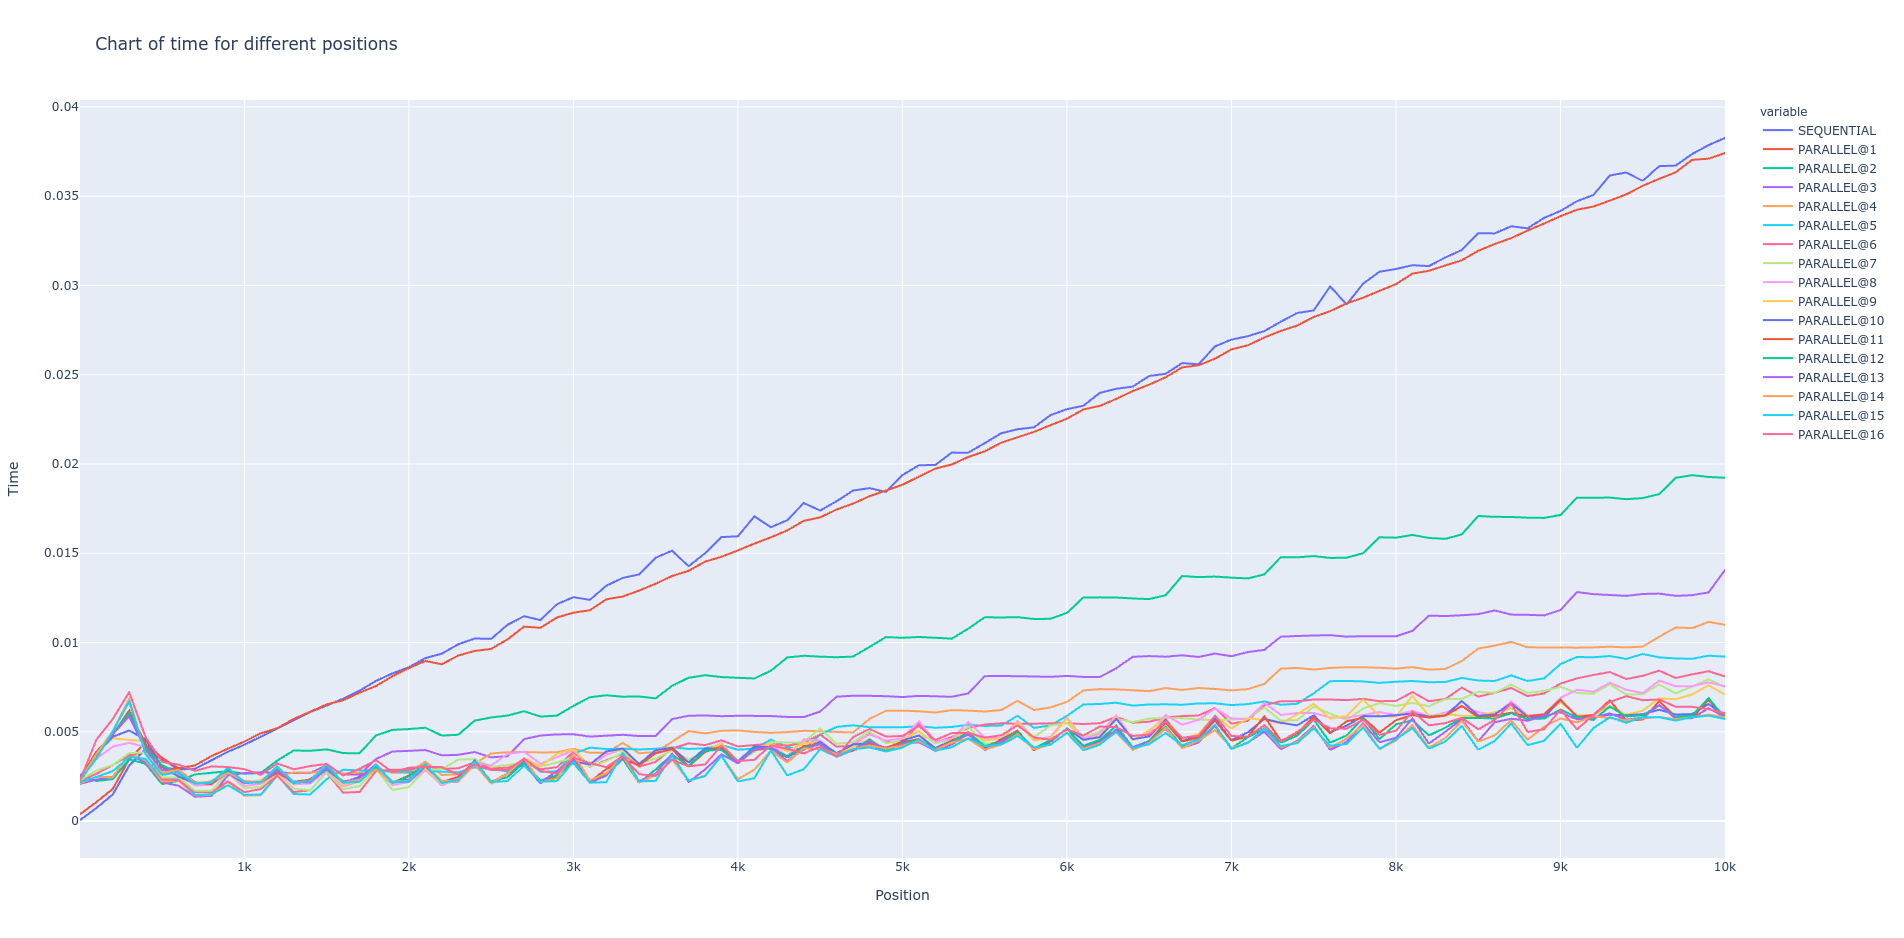
\includegraphics[width=1.0\linewidth]{./img/positions-10k.png}
    \end{center}
        \caption{The times measured for the first 10000 positions}
    \label{fig:position-10k}
    \end{figure*}

    Other important evaluations can be made by observing the speedup charts, showed in Figure
    \ref{fig:speedup} for passwords found at position 1M and in Figure \ref{fig:speedup-5k}
    for passwords found at position 5k:

    \begin{itemize}
        \item when the password is found later in the dictionary using more threads gives
              better results but that stops at around 15 threads, thus we can say that that
              is the optimal number for running this solution on this machine; it is
              expectable that this number will be higher when CPUs with more cores
              are used.
        \item when the password is found sooner in the dictionary the parallel solution gives
              anyway better results than the sequential solution but those results stops
              getting better when using more than 6-8 threads and even start to degrade when
              using more than 14 threads.
    \end{itemize}

    \begin{figure*}
    \begin{center}
    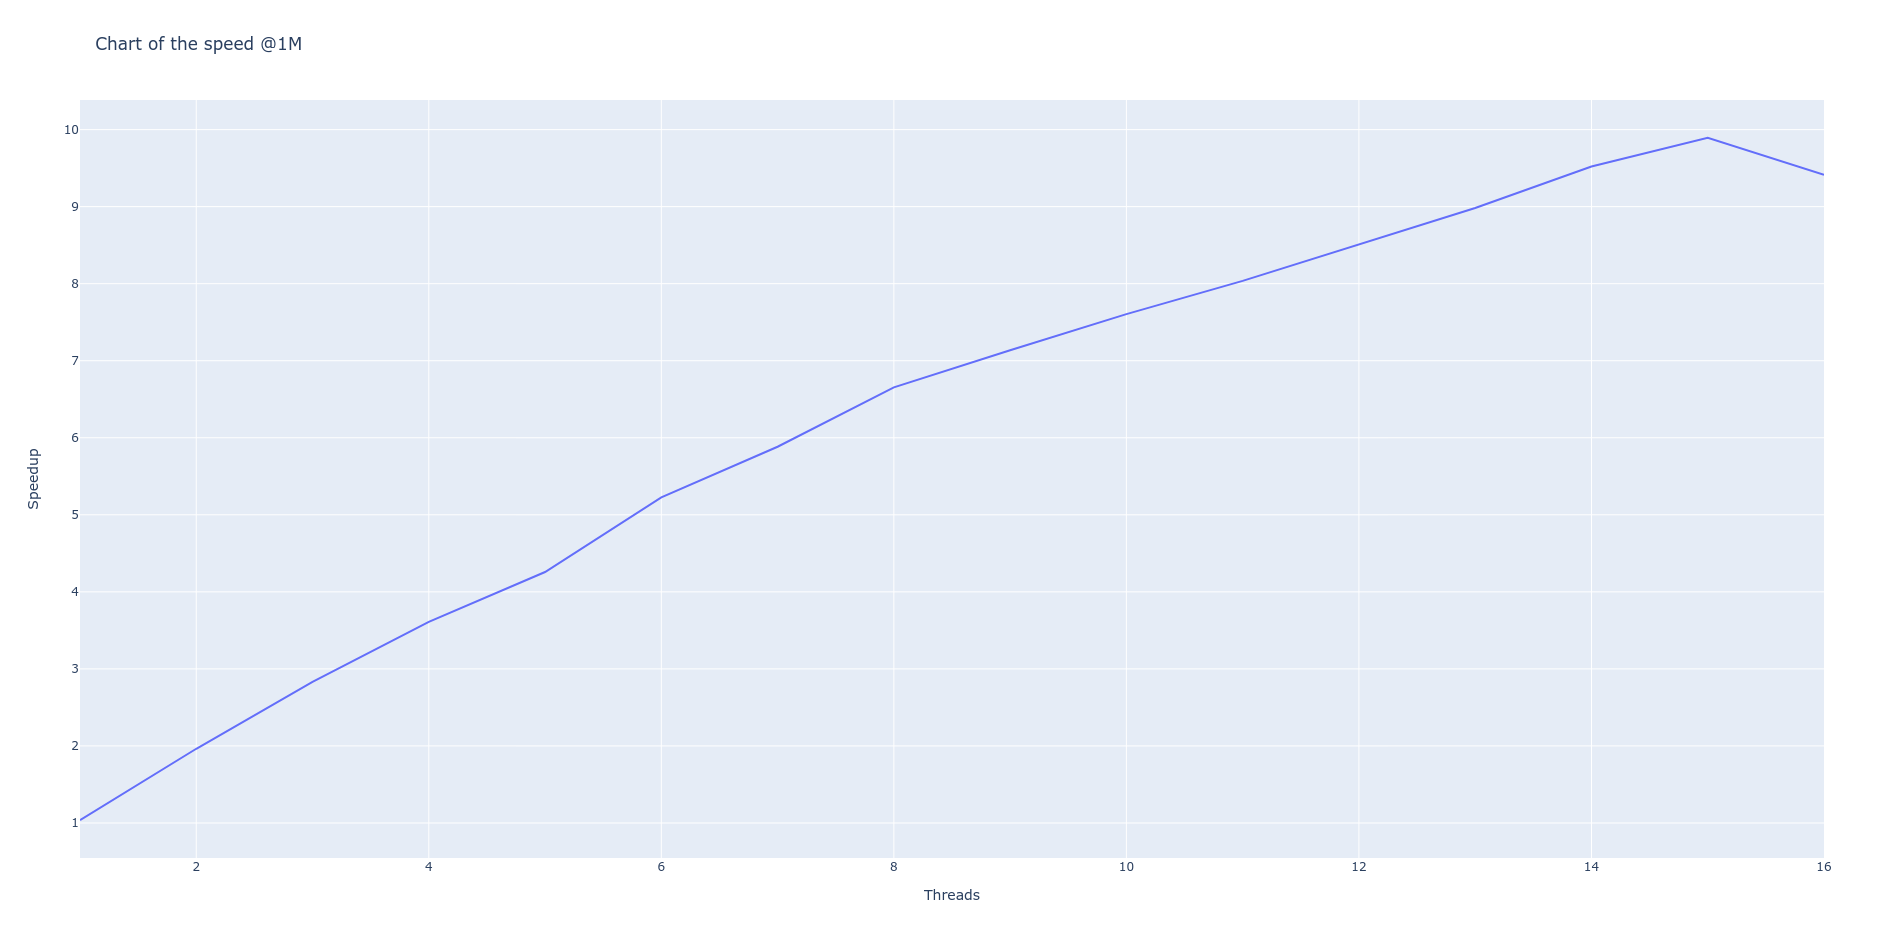
\includegraphics[width=1.0\linewidth]{./img/speedup.png}
    \end{center}
        \caption{Speedup searching for the password at position 1M}
    \label{fig:speedup}
    \end{figure*}

    \begin{figure*}
    \begin{center}
    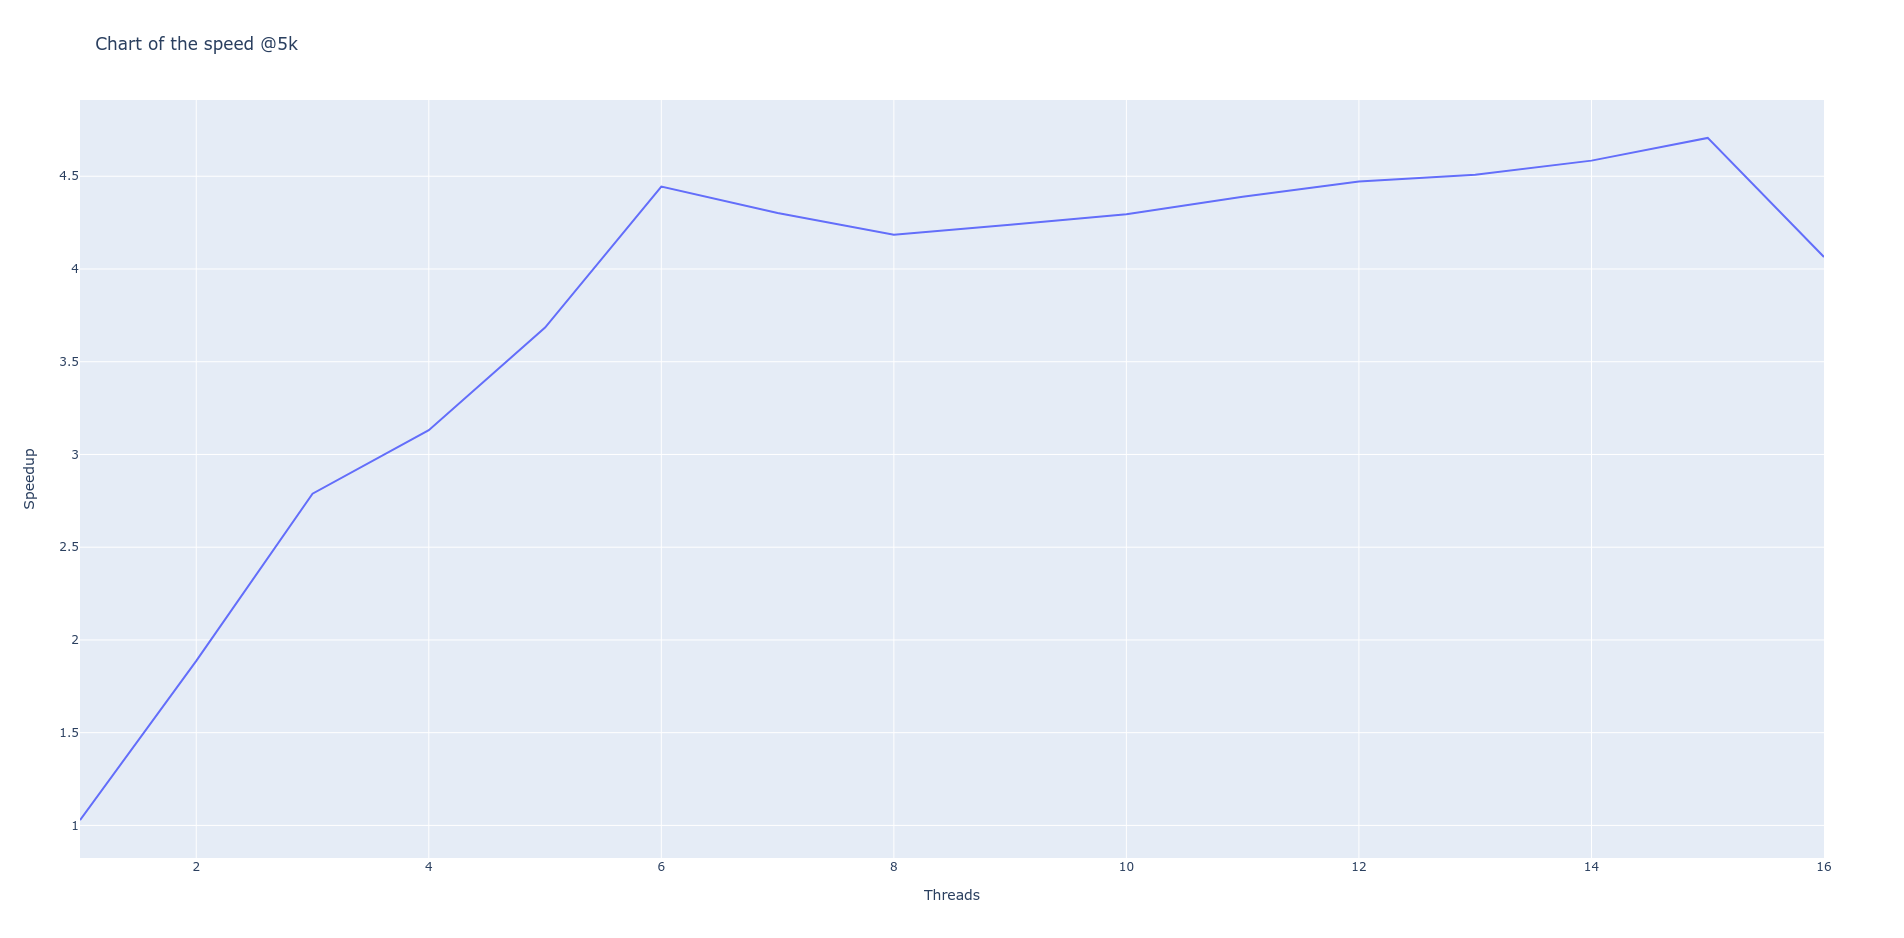
\includegraphics[width=1.0\linewidth]{./img/speedup-5k.png}
    \end{center}
        \caption{Speedup searching for the password at position 5k}
    \label{fig:speedup-5k}
    \end{figure*}

\clearpage

\nocite{*}
\twocolumn
\bibliographystyle{ieee}
\bibliography{project_report.bib}
\onecolumn

\end{document}
